\chapter{Konzept} 	% engl. Preface


\section{Analyse}

Zu Beginn des Spiels muss die Zeitanzeige auf null gesetzt werden, also 00:00 anzeigen. Auch die Anzeige für den Spielstand muss null zu null gesetzt werden. Das Spiel und somit der Ablauf der Zeit soll dann per Knopfdruck gestartet werden. Die aktuelle Zeit sowie der Spielstand sollten dabei stets im Hauptspeicher hinterlegt sein. Neben der Option das Spiel per Knopfdruck zu starten, soll man die Zeit anhalten können. Zudem können beide Anzeigen zurück auf 0 gesetzt werden. Auch das Zählen der Tore ist über die Steuerung möglich. Dabei kann die Zahl der Tore sowohl um eins erhöht als auch um eins erniedrigt werden. 

Zur Anzeige der Zahlenwerte dienen 7 Segment Anzeigen. Diese dienen jeweils als Pärchen als verschiedene Anzeigen. Die Aufgaben eines Pärchens ist einmal Anzeigen eines Spielstandes oder das anzeigen der aktuellen Zeit.

Zur Steuerung wird ein Simple Keypad genutzt. Dieses hat acht Knöpfe, die jeweils mit den oben beschriebenen Funktionen belegt werden und so die Anzeigen steuern können.

\begin{figure}[h]
	\centering
	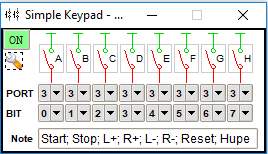
\includegraphics[width=0.9\textwidth]{Button} 
	\caption{Abbildung Simple Keypad  Eigener Screenshot }
	\label{fig:Button}
\end{figure}

\begin{figure}[h]
	\centering
	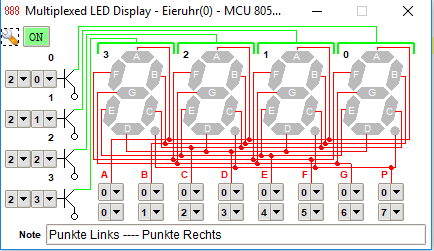
\includegraphics[width=0.9\textwidth]{Spielstand} 
	\caption{Abbildung Spielstand  Eigener Screenshot }
	\label{fig:Spielstand}
\end{figure}

\begin{figure}[h]
	\centering
	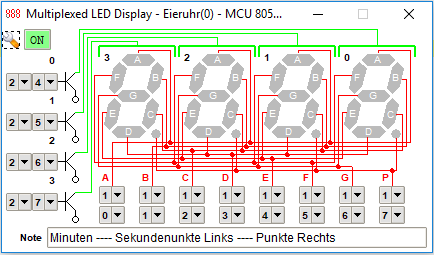
\includegraphics[width=0.9\textwidth]{Zeit} 
	\caption{Abbildung Spielzeit  Eigener Screenshot }
	\label{fig:Zeit}
\end{figure}

\section{Programmentwurf}

Die Ergebnisse der Analyse sollen nun in einen Programmentwurf umgesetzt werden. Zu Beginn werden dafür den verschiedenen Elementen, der in der Analyse beschrieben Hilfsmittel, bestimmte Speicherbereiche zugewiesen.
\begin{table}[H]
	\centering
	\caption{My caption}
	\label{my-label}
	\begin{tabular}{lll}
		Speicheradressbereich & Inhalt  \\
		60h-63h & Punkte  \\
		64h-67h & Zeit   \\
		2Fh & Funktionen  
	\end{tabular}
\end{table}

Neben der Festlegung der Speicherbereiche, wird die Hardware über die I/O Ports verbunden. Dabei werden die folgenden Ports für die jeweiligen Anzeigen genutzt:
\begin{itemize}
	\item Minuten und Sekunden anzeige für ein Fußballspiel (Port0)
	\item Punkte Anzeige für jedes Team  (Port1)
	\item Ansteuerung der jeweiligen 7 Segmentanzeige (Port2)
	\item Simple Keypad zur Steuerung (Port3)
\end{itemize}  


Wenn das Programm aufgerufen wird, kann der Ablauf der Zeit mit dem Simple Keypad eingeleitet werden. Dafür muss der erste Knopf auf dem Keypad einmal gedrückt werden. Er wird somit geschaltet und nimmt den Wert 0 an. Anschließend muss er noch einmal betätigt werden, um die Zeit zu starten, da nur beim Schalten von 0 auf 1 eine Veränderung des Wertes festgestellt wird. Das gleiche gilt für die anderen Knöpfe des Keypads. Auch sie müssen je von 0 auf 1 geändert werden um eine Veränderung zu bekommen. 

Um das Hochzählen der Zeit genau kontrollieren zu können wird ein Timer implementiert der während dem Ablauf des Programmes automatisch hochzählt. Die Zahl wie oft der Timer hochzählt, ist dabei so gewählt, dass genau eine Sekunde vergeht bevor die Anzeige noch einmal hochzählt. Dieser Wert ist aufgrund der Geschwindigkeit der IDE bei unserem Programm kleiner gewählt. 

Das Hauptprogramm läuft eigentlich unabhängig vom Timer selbst. Allerdings kommt es sobald der Timer fertig hochgezählt hat, es also zu einem Überlauf kommt, zu einem Interrupt, durch den das Programm unterbrochen wird. Erst nachdem dieser Interrupt vom Timer beendet wird, kann das Programm weiterlaufen. 

 
 
 